\documentclass[11pt,a4paper]{article}

\usepackage{color,graphicx,listings,wrapfig,hyperref,algpseudocode,algorithm,natbib}
%\usepackage[margin=2cm]{geometry}
\usepackage{amsmath,subcaption}
\usepackage[toc,page]{appendix}

\newcommand{\BigO}[1]{\ensuremath{\operatorname{O}\bigl(#1\bigr)}}

\graphicspath{{./img/}}

\begin{document}
\title{Masters project}
\author{Michal Kawalec}
\maketitle

\section{Introduction}

% This is just a mock introduction, will need to be changed at the end
In this thesis we study the behaviour of a flow of fluid in a pipe.
As can easily be imagined, having a proper model that provides us with an ability to discover its dynamics with little computational expense would enable us to have a better understanding of how the flow occurs and changes to turbulence.
Before discussing the model though, we present a firm theoretical base on which further understanding will be built.

\subsection{Transition to turbulence}
Discovering when and how a divergenceless fluid transits from linear flow to a turbulent one is of great importance in many areas of life and industry.
As the turbulent state produces a much increased drag than a simple parabolic profile, being able to predict and minimize the frequency of its occurrence would enable us to transport many liquid goods like oil more efficiently.
This problem of when and how turbulence appears has been asked for quite some time now, starting with the classic papers by Poiseuille\cite{Poiseuille40} and Reynolds\cite{Reynolds83}.
Reynolds has introduced a concept of a Reynolds number, which was experimentally determined to indicate the expected bulk behaviour of a fluid as its speed increases.
Reynolds number is expressed in terms of the mean flow speed \(u\), pipe diameter \(d\) and viscosity of the fluid in question \(v\) as \(Re = ud/v\).
Reynolds discovered that, for his experiment, it was possible to carefully maintain the laminar flow up to \(Re\) of \(12000\).
Above that number, the turbulence seemed to occur by itself, and he was unable to control it.
Interestingly, the point at which the turbulence was possible to be triggered by an external stimulus was much lower, around \(Re = 2000\).
Other literature places this lowest transition point in the range of 1760 to 2300\cite{Kerswell05}.
One could wonder what is the reason behind this spread of values in different experiments.

As we now know, for a liquid flowing in a pipe, the laminar profile is stable at any Reynolds number\cite{Eckhardt07}.
Therefore in order for the flow to transit to a turbulent situation a stimulus needs to be applied to the pipe, usually in form of a fluid injection or suction\cite{Darbyshire95}.
In order for the turbulent flow to be observed the perturbation needs to be strong enough for disturbance to not decay and produce at least an instant of turbulence in the fluid flow\cite{Salwen80}\cite{Meseguer03}.
Because of a variation in perturbation strengths and differing methods in experiments made a range of transition points was determined.
Additionally, it was noticed that the higher a Reynolds number for a flow, the lower the strength of a perturbation that needs to be applied to turn the flow turbulent\cite{Hof03}.
The differing perturbation strength is also the reason for the maximum Reynolds number at which a laminar flow can be sustained.
Certain perturbations are impossible to get rid of in a real experimental setting, like ground vibrations from a distant highway or impurities in the pipe geometry.
We will later discuss the exact nature of the perturbations applied and dependence of the points of transition on them.

Surprisingly, in pipe flow there is no state with simple spatial or temporal structures between the laminar and turbulent flow\cite{Eckhardt07}.
This is in contrary to other flows and their corresponding intermediate structures, like rolls in Reyleigh-Benard or Taylor vortices in Taylor-Couette.
There are however two types of complex transitional flow states, existing between complete turbulence and laminar flow.
As described by Wygnanski \& Champagne\cite{Wygnanski73} in the \(Re\) range of 2000 to 2700 there exist `turbulent puffs'.
These structures have a well defined rear interface that divides a laminar flow at the back and a localized area of chaotic motion in front.
The structure moves with a speed just a bit lower from that of a mean flow, therefore being quite localised and rarely increasing its volume considerably over the starting dimensions.
Ahead of a puff there is an indeterminate front interface followed by a usual, undisturbed flow that did not have a chance to be disrupted.
Because of the speed of the puff being similar to that of the flow and because of the well defined rear interface, a puff does not induce turbulence in the pipe as a whole, and after it moves forward with the flow, the subsequent motion in the place where disturbance happened is laminar.
At higher Reynolds numbers of \(Re > 3500\), perturbing the flow with an intensity too low to trigger full blown turbulence introduces `turbulent slugs'.
They extend throughout the whole cross-section of the pipe and have well defined interfaces on both sides.
Because the speed of their rear interface is lower than the mean flow speed, and the speed of the front interface higher, they can extend through most of the pipe.
As \(Re\) increases to values greater than \(10000\) the speeds of the front and rear interfaces approach 1.5 and 0.5 of the average speed of the flow respectively.
Despite that `pipe consuming' behaviour, a slug is still a localised phenomenon, and disappears travelling with the flow.

It is not only the transition from the laminar flow to turbulence that can be interesting and full of surprises.
It turns out that the turbulent state can decay into laminar flow by itself and with no clear precursors, which is a property of a flow existing in both the numerical simulations\cite{Brosa89}\cite{Faisst04} and experiments\cite{Darbyshire95}\cite{Hof04}\cite{Mullin06}.
Additionally, such flow patterns are observed in our one dimensional model, as will be discussed later.

A common device for understanding complex mechanical systems is to consider them in their state space, which in case of a fluid flow in a pipe\cite{Lanford82} is a space of all velocity fields that can possibly occur as the flow undergoes various transitions.
Because we know that the parabolic profile is stable\cite{Eckhardt07} and will never turn into turbulence by itself, it is a fixed point and an attractor in the phase space.
As the Reynolds number increases the strength of the attraction decreases, thus making it much more likely for the flow to escape the basin of attraction and become turbulent.
This is evidenced in results of experiments and simulations (CITE) showing that increasing Reynolds number decreases the perturbation required for triggering the turbulence.
If the turbulent states were attractors\cite{Guckenheimer86}\cite{Lanford82}, all states close to the turbulent region would evolve towards the turbulence.
However, we know both from the chaotic dynamics of the turbulent regions and from the fact turbulence can decay with no clear precursors that there must be chaotic elements\cite{Guckenheimer83} like horseshoes connected to the laminar profile in some ways.
Such structures, that explain the dynamics of the turbulent motion, are known as chaotic or strange saddles.
It is important to note that motion close to such saddles has a positive and important Lyapunov exponent, which in effect removes any notable correlation in the phase space trajectories.
With uncorrelated trajectories, the probability of escaping from the saddle is constant in time.

An analogy that we think enables one to intuitively gasp the motion of a chaotic system in its state space is to consider a particle bouncing in an irregular box\cite{Ott93}.
As long as the box is not of a simple, symmetric shape like an ellipsoid or a cube, the dynamics of the particle will be chaotic, and thus representing our system well\cite{Ott93}.
To make this scheme dissipative and not energy conserving, as is the case with a flow of real fluid, we can introduce a dissipative term of any origin and a motor powering the particle.
The model is still incomplete at this stage, as we haven't specified how such motion could decay.
Cutting out a hole of an appropriate size in a wall of the box would provide us with an opportunity of accommodating for this case: if the particle escapes the box, we assume that the system had decayed.
Before hitting the hole the particle is going to bounce around in a random fashion.
Its motion will exhibit a positive Lyapunov exponent, which will cause it to quickly loose correlation between the starting conditions.
Therefore, as in the real turbulent motion, the probability of hitting the wall will be constant, that means proportional to the ratio of the area of the hole and the total surface area of the box.
There is an even deeper analogy to the real case here.
Because the influence of the Lyapunov exponent increases as the time progresses, the chance of the fast decaying cases of the particle hitting a wall soon after being released will diverge from the constant probability case existing for longer lasting motion.

This seemingly simple model is surprisingly close to what actually happens in a pipe flow.
Apart from providing us with an intuitive understanding of state space dynamics of turbulence and its decay it implies that the distribution of lifetimes has to be exponential, which stems from the positive Lyapunov exponent causing the probability of hitting a wall to be constant.
As noticed above, this will not be true for fast decaying motion, for which a departure from the exponential decay will be noted.
The experimental and theoretical grounding of this lifetime distribution will be discussed later.
So far, it was only possible to determine an exact value of the Lyapunov constant for pipe flows in numerical simulations\cite{Faisst04} as the process requires a control of starting conditions to a degree not yet possible in an experimental setting.


\subsubsection{Experiments}
In experiments the transition to turbulence is triggered by either injecting in or sucking out a certain amount of liquid from the flow.
The change in the amount of liquid perturbs the parabolic profile of a linear flow and causes it either to become turbulent or not.
If the fluid doesn't become turbulent, the perturbation decays and no persistent turbulence is noted.
Darbyshire \& Mullin\cite{Darbyshire95} investigated what amplitude of perturbations needs to be applied to a parabolic profile to trigger the transition to turbulence for a pipe flow.
They discovered not only that for the neighbouring points (up to the experimental resolution) the effect of applying the perturbation can be strikingly different, but that for the same points the transition sometimes occurred and sometimes didn't.
Additionally, there seemed to be no way of determining (except from a rough estimate) if a given disturbance is going to cause a transition of turbulence, or will decay to the laminar state without inducing the disturbance.

\begin{figure}[h!]
    \centering
    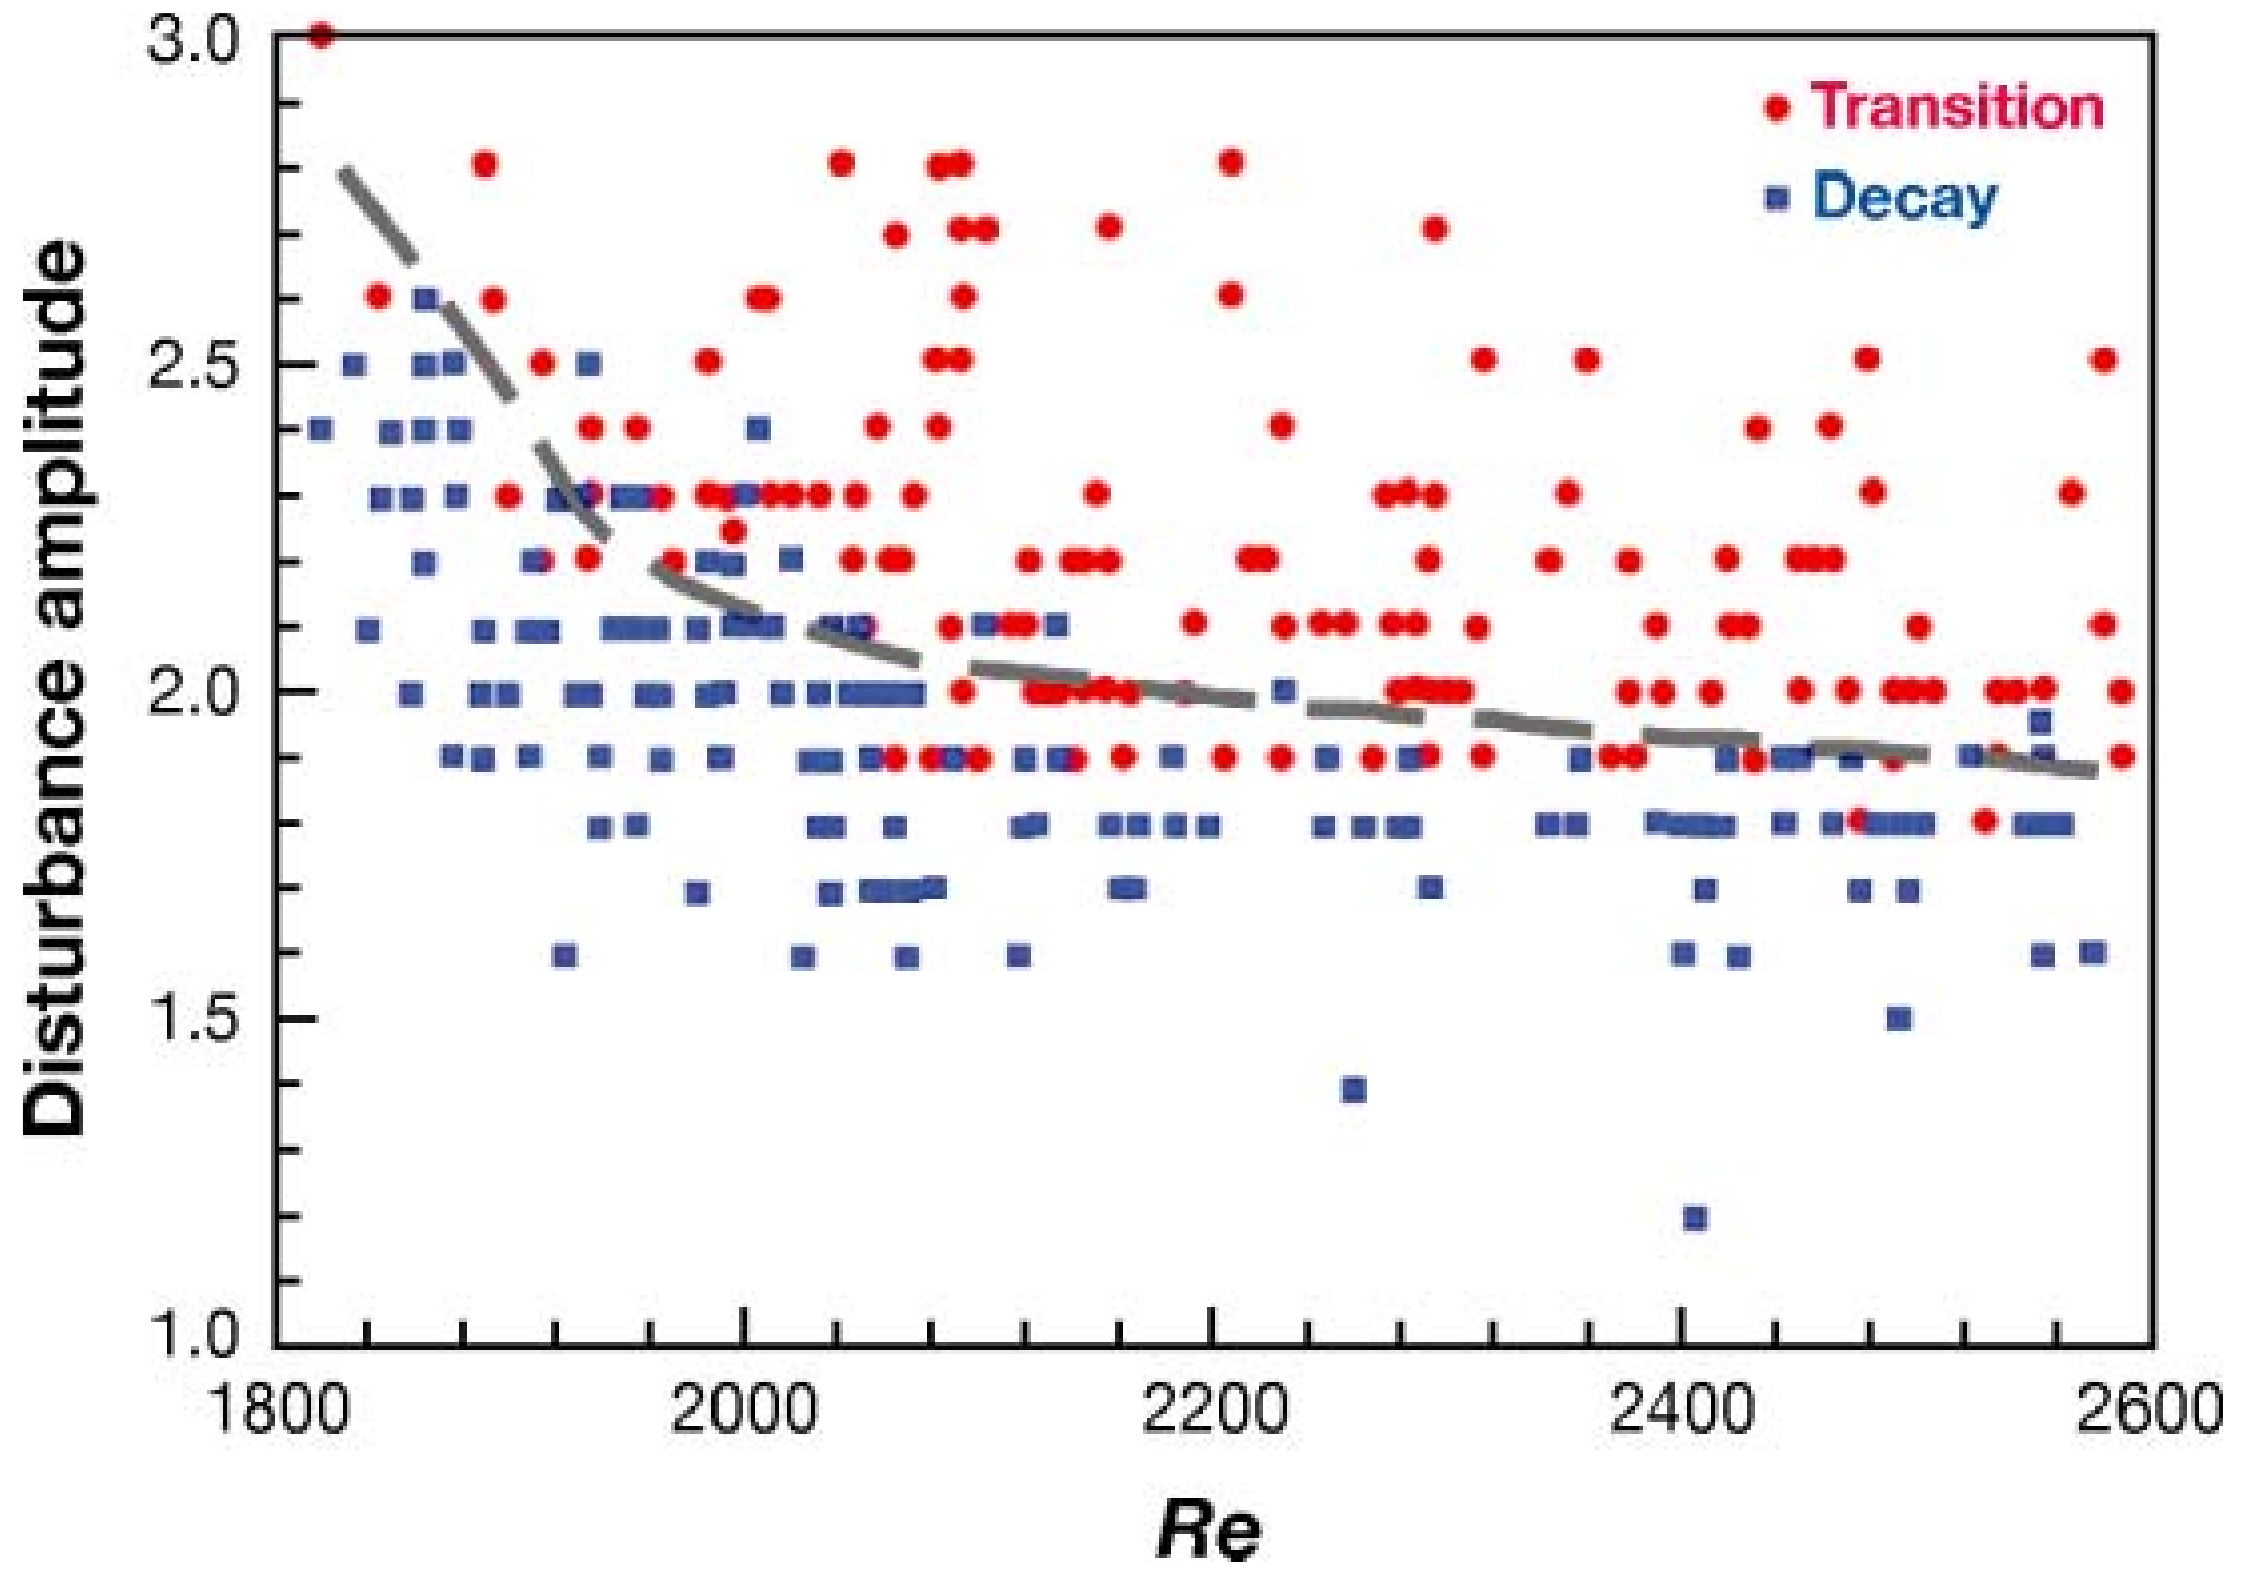
\includegraphics[width=0.95\textwidth]{darbyshire95.png}
    \caption{Turbulence transition results obtained by Darbyshire \& Mullin\cite{Darbyshire95}, reprinted and coloured by Eckhardt et al.\cite{Eckhardt07}}\label{img:darbyshire_plot}
\end{figure}

Despite that though, an approximate line can be drawn that separates the `mostly turbulent' area from the `mostly decaying' one and provides us with a relation that the higher the Reynolds number the smaller disturbance is required to trigger turbulence.
Of course this relation needs to be taken with a pinch of salt, as it is only correct on a coarse scale\cite{Eckhardt07}.
Any experiment has physical limits on its accuracy and so it is often only possible to use numerical simulations to investigate the effects of slight changes in starting conditions.
In a simulation one has perfect control (up to numerical accuracy and the algorithm chosen) over the starting conditions and the evolution of the simulation and thus much more accurate results are possible to be achieved.
In concert with the experimental results a simulation by Faisst \& Eckhardt\cite{Faisst04} shows that perturbation amplitudes very close to one another produce turbulence with strikingly different lifetimes.
Their results also confirm the inverse relation between the Reynolds number of a flow and strength of a perturbation required to trigger turbulence.
This relation is again confirmed by experiments in the ranges of Reynolds numbers from \(2000\) to \(20000\), where the `coarse-scale' critical amplitude dependence on \(Re\) as \(1 / Re\) is reported\cite{Hof03}\cite{Hof04}\cite{Draad98}.

\subsubsection{Lifetimes}
It is generally agreed that because of the strong variability of lifetimes with changing initial conditions, it is more useful to look at the lifetimes in bulk, focusing on certain statistical properties of them, such as the survival probability at different times from the instant when the perturbation was introduced.
Because of the positive Lyapunov constant in the evolution of the system through the phase space, the probability of decay to the laminar state is independent of time, just as in our example of a particle in a box.
Because of the decay probability being constant in time, the distribution of lifetimes is an exponential\cite{Kadanoff84}.
The experimental data confirms this theoretical prediction and exponential distribution of survival probability is indeed observed.
Such a distribution implies the earlier mentioned property of the turbulent state to be a chaotic saddle in the state space.
As well as being supported by experiment, numerical simulations also produce exponentially decaying survival probabilities\cite{Eckhardt02}.
Additionally, same functional form of the dependence was found in plane Couette flow by Bottin \& Chate\cite{Bottin98} experimentally, and numerically by Eckhardt\cite{Eckhardt02}.

\begin{figure}[h!]
    \centering
    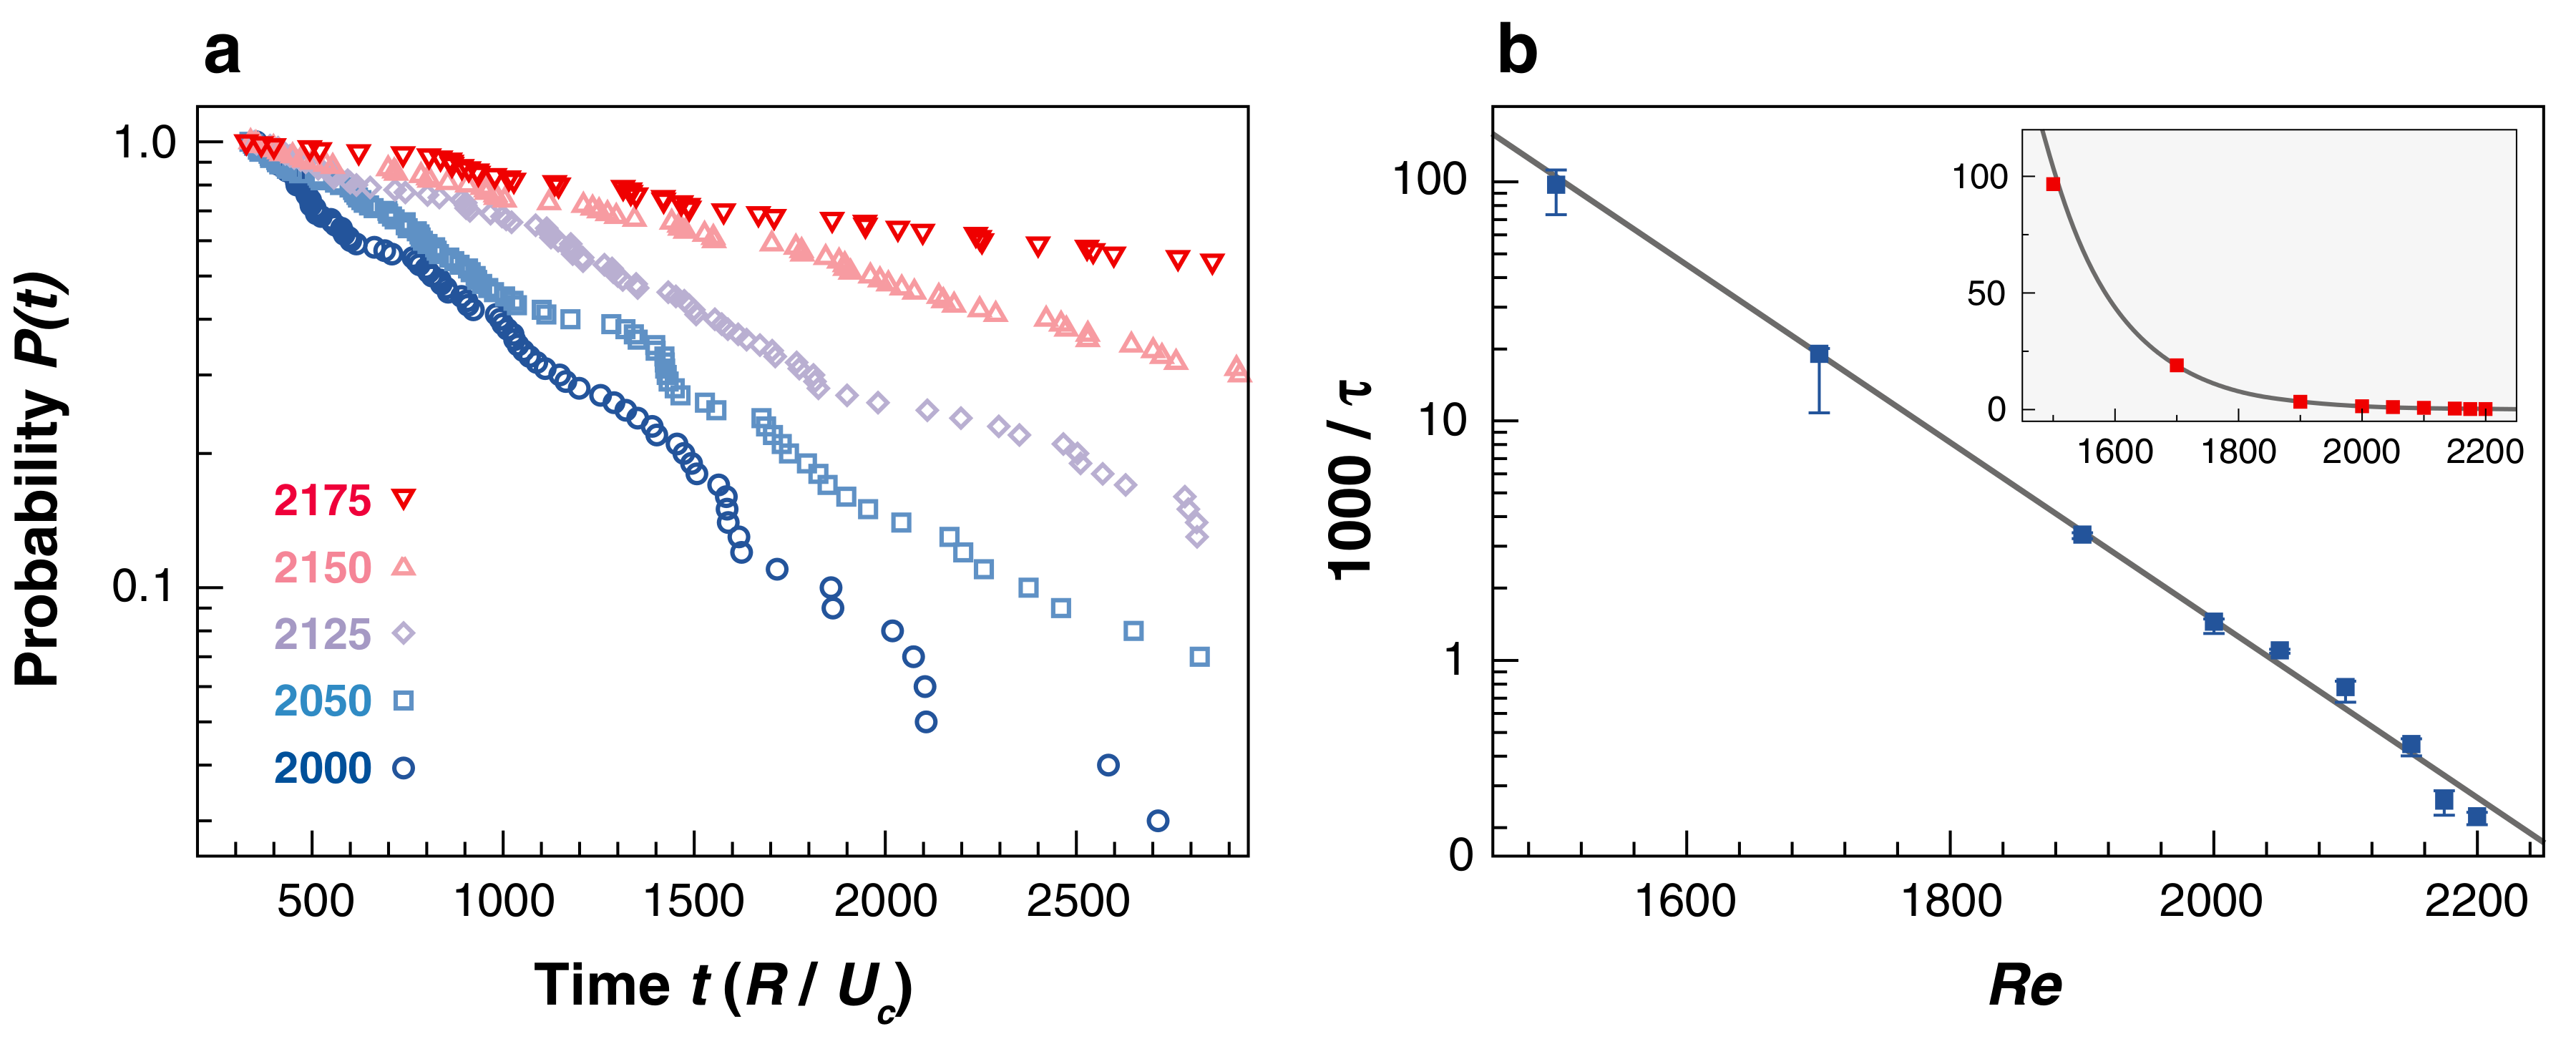
\includegraphics[width=0.95\textwidth]{decay_prob.png}
    \caption{Survival probabilities for different Reynolds numbers as determined by Direct Numerical Simulations by Eckhardt et al\cite{Eckhardt02}.}\label{img:decay_plot}
\end{figure}

Naturally, in the above cases we are talking about the tail of survival probability distribution, as at short lifetimes the evolution is influenced strongly by starting conditions and thus deviate from the exponential fit quite markedly in some cases.
Using the data we have from the numerical simulations we can tell that the characteristic time of the probability distribution increases quite drastically with an increasing Reynolds number.
While there is no theoretical prediction to the nature of the dependence of this time on the Reynolds number, the most recent experiments performed in long pipes suggest that the characteristic time does not diverge, but increases exponentially with Reynolds number.
This is in line with the results of numerical simulations which, in a limited \(Re\) range, have also shown an exponential increase of the characteristic time.

\subsubsection{Exact coherent states}
As much as the motion of a system in a turbulent state is chaotic, we know now that there exist simpler, regular solutions to the equations of motion.
Because we know that the turbulence is a chaotic saddle, different researchers have tried to find these saddle states around which the motion evolves\cite{Clever92}\cite{Clever97}\cite{Nagata90}\cite{Faisst00}.
Finding these states that guide the spatial and temporal evolution of a flow in a pipe may help with understanding the nature of flow better.
Because of the lack of inversion symmetry in the laminar profile of a pipe flow, the simplest coherent solutions to the equations of motion take form of travelling waves.
An example of such a travelling wave is presented on Image~\ref{img:stat_states}, arrows indicating fluid flow in place of the cross-section.

\begin{figure}[h!]
    \centering
    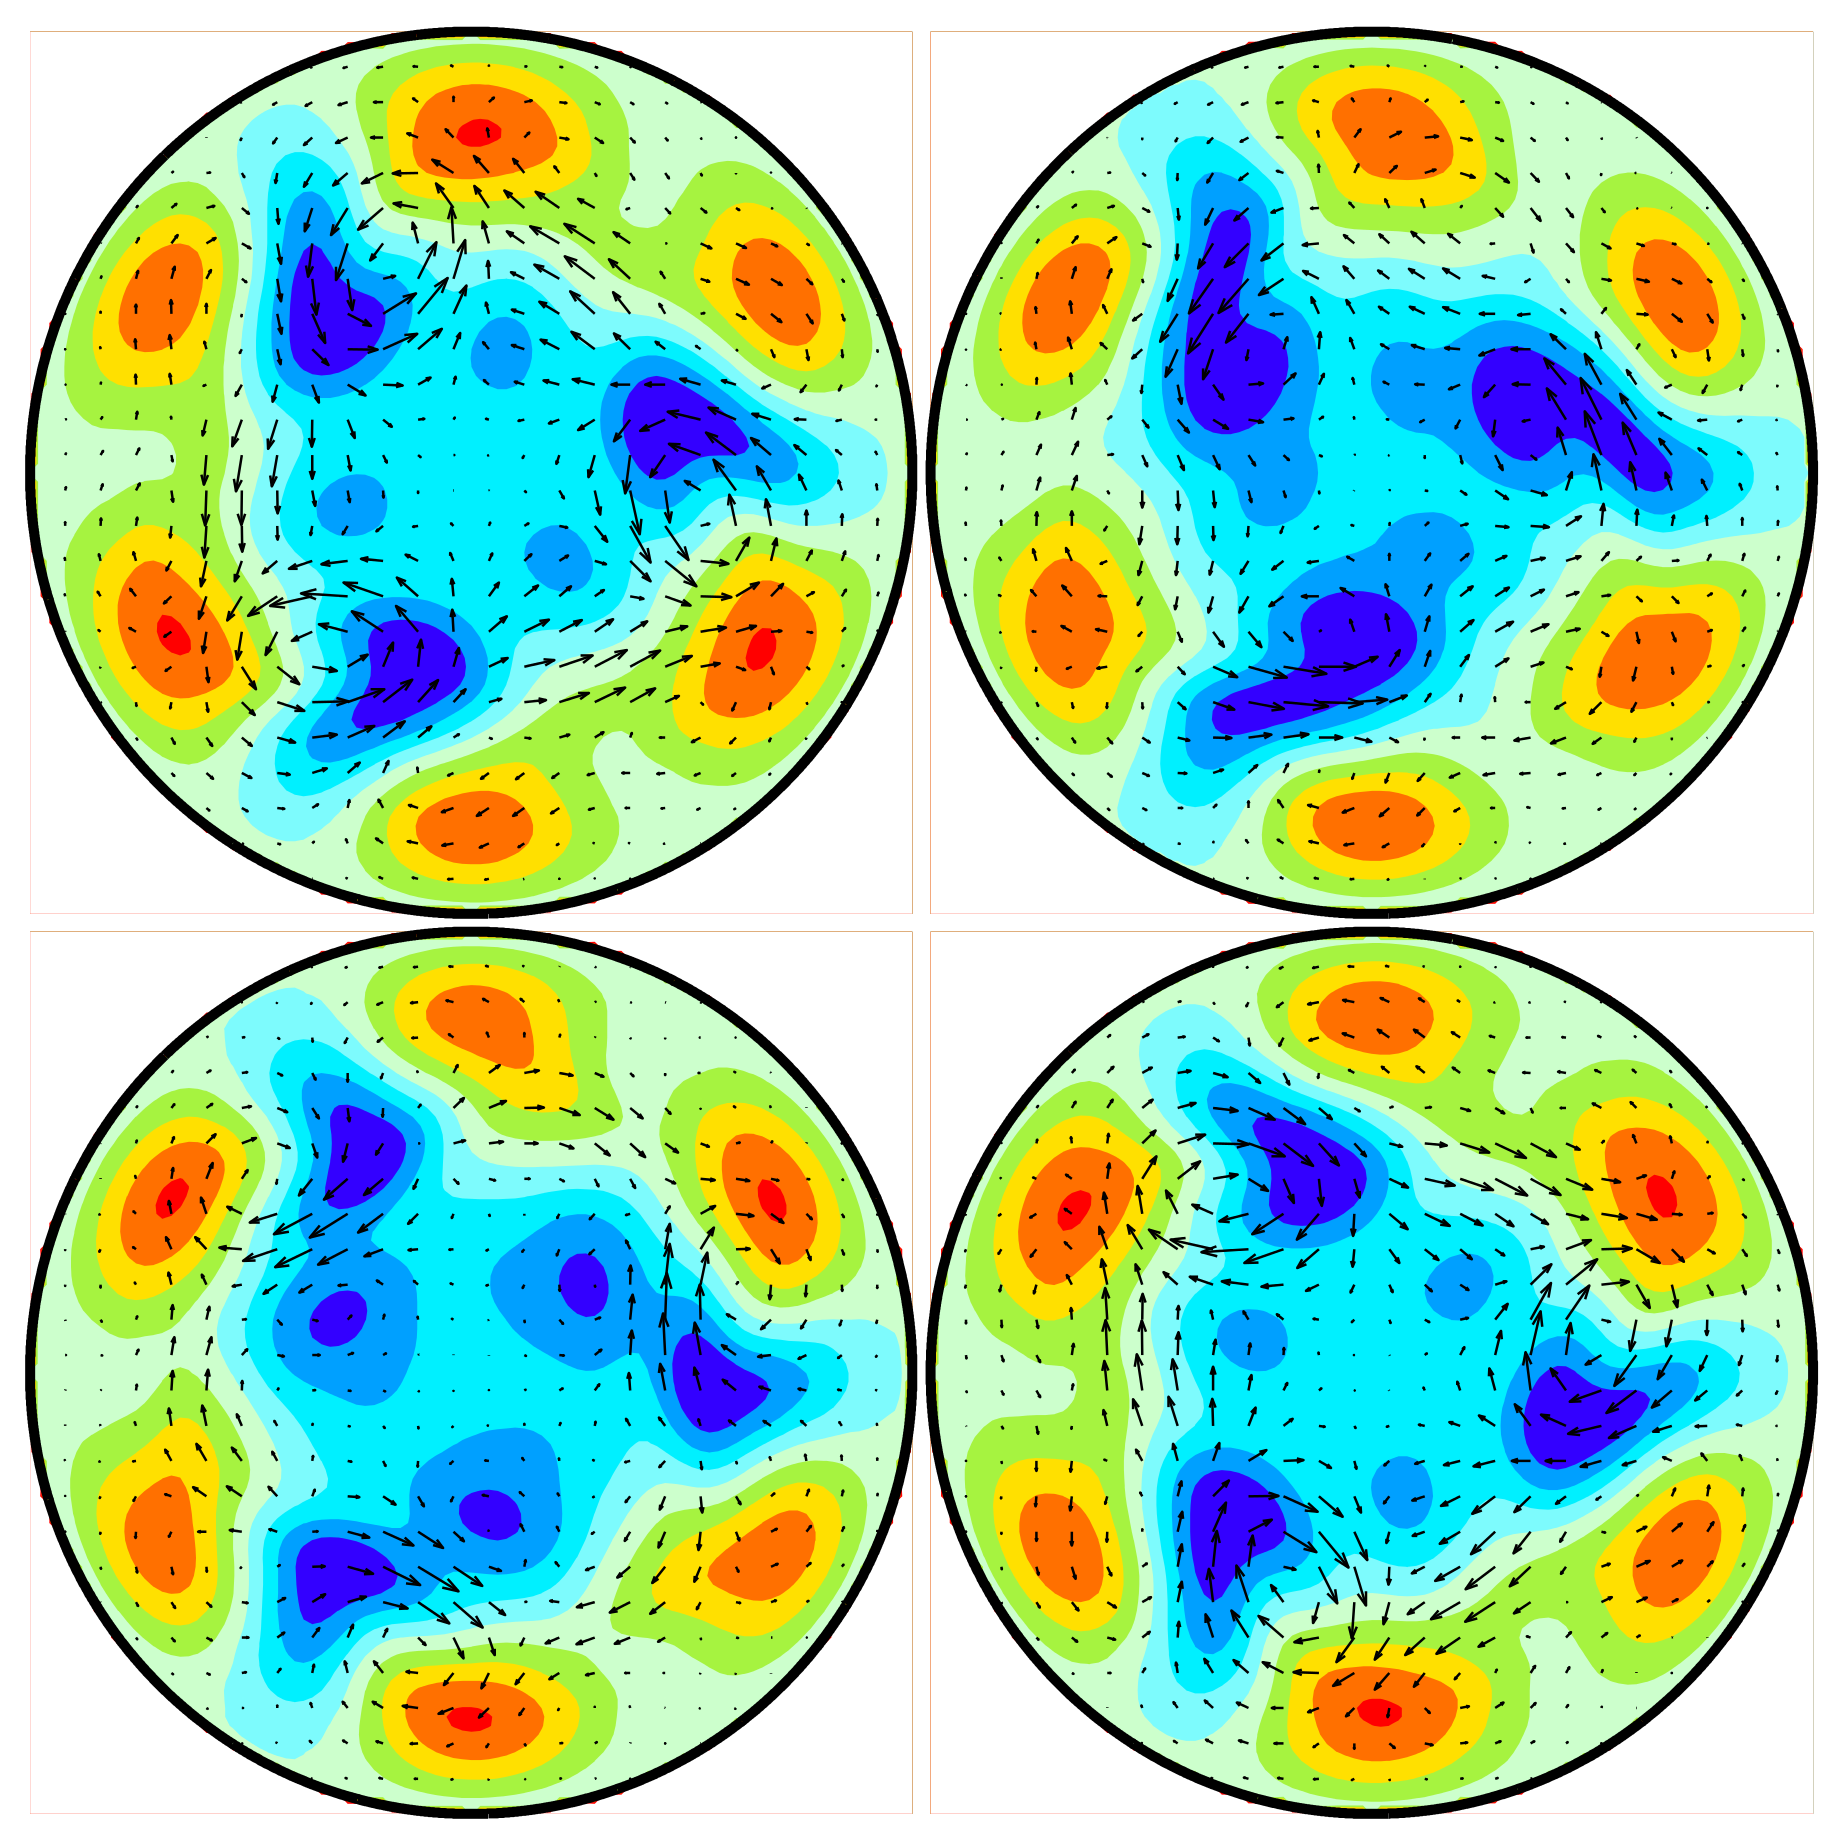
\includegraphics[width=0.65\textwidth]{stationary_states.png}
    \caption{An example of a stationary wave, shown here in the first half of its period (the other half is inverted in the horizontal axis). Each cross-section shows a snapshot of the wave every $1/6$ of its period, as found by Faisst \& Eckhardt\cite{Faist08}.}\label{img:stat_states}
\end{figure}

The waves that have been found contain from two to five `vortex pairs that generate high-speed streaks close to the walls and low speed streaks in the centre'\cite{Eckhardt07}.
As the time passes, the high-speed streaks evolve very little, with some minor change in their intensity, whereas the low-speed ones move around the centre of the flow quite considerably.
States strikingly similar to the ones predicted by the simulation are observed by means of stereoscopic particle image velocimetry\cite{How04etal}.
The technique requires addition of light-reflecting particles and measuring their positions in a thin cross-section of the flow produced by light from a pulsed laser.
Difference between the observed states and the ones predicted by the simulation is due to both the dissipative nature of a flow and the fact that a trajectory of the system in a state space will lead close, but not through the stationary states.

An important idea to stress again is the fact that the survival probability for a chaotic saddle, such as the one spanned by the coherent state will be an exponential.
That, when one thinks about the analogy of particle in a box, implies that movement around a chaotic saddle will always decay, with a lower or higher component of an exponential.

\begin{figure}[h!]
    \centering
    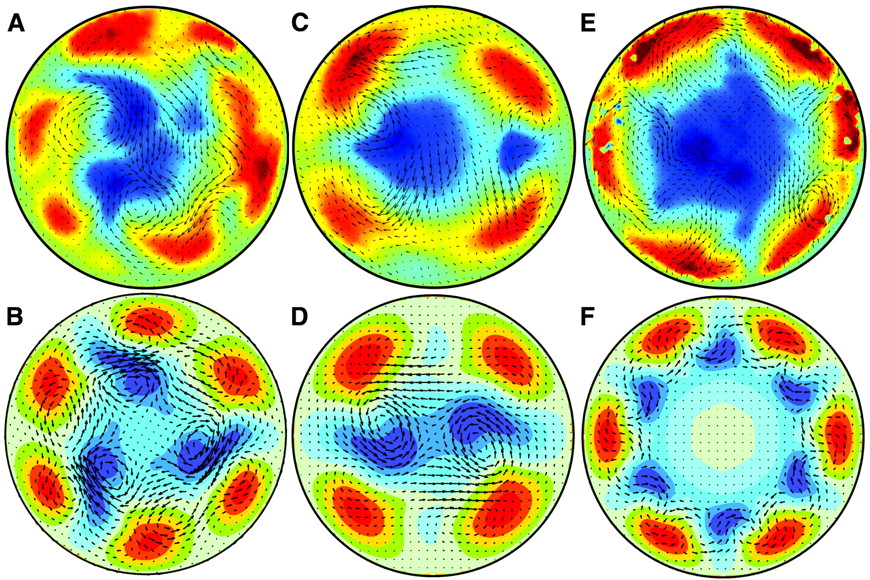
\includegraphics[width=0.95\textwidth]{experiment_vs_simulation.jpg}
    \caption{Comparison of the states predicted by the means of numerical simulation, on the bottom, and states observed with PIV\cite{Hof04etal}.}\label{img:ex_simu}
\end{figure}

\subsection{Drag reduction}

It turns out that addition of particles into the flow quite strikingly changes its behaviour and subsequent evolution in the state space.
It has been known since the 1940s\cite{Toms49}\cite{Mysels72} that addition of very limited amounts of polymers to water heavily reduces its its propensity to become turbulent and enables laminar flows at higher Reynolds numbers.
Additionally, once the motion becomes turbulent, the polymer additive reduces drag by around 80\%\cite{Sreenivasan00}.
Later it was noticed that elasticity displayed by the polymer is not required for a substantial modification of the flow dynamics\cite{Pashkewitz04} and materials such as paper or cloth pulp\cite{Radin75}\cite{Robertson57}, asbestos\cite{Mccomb85} and colloidal crystals\cite{Pirith72}\cite{Radin75}.
Drag reduction caused by the non-elastic additives is less pronounced than that caused by polymers of various kinds.
Even though certain methods have been proposed\cite{Pashkewitz04}\cite{Lee74} of combining properties of elastic and non-elastic additives to achieve stronger drag reduction, we will not discuss it here, as it is not a focus of this thesis.

This effect is widely applied in fluid transport in pipelines\cite{Graham04} and was considered to be used for faster sea transportation\cite{Dimotakis03}, before the idea was dropped because of costs concerns.
The reason why polymers were even considered to be worthy of being used in increasing speed of vessels on an open sea is that they are extremely potent drag reducers.
Even concentrations as low as parts per million produce visible effects.
An interesting property of the polymeric drag reduction is the existence of a phenomenon called the maximum drag reduction (MDR).
Once enough polymer is added to the solution, drag reduction can be observed.
As the concentration is increased, DR increases proportionally, until the point when it reaches a limit.
Adding more polymers cannot decrease the drag further.

\subsection{Motivation}
In this thesis we want to implement and test a simple, one dimensional model for turbulent flow and drag reduction in a pipe.
Because of a significantly reduced computational requirements, it is possible to execute the model for much longer times, domain sizes and numbers of runs than is possible with full direct numerical simulation of a fluid with embedded polymers.
We will compare the results produced by the model with the ones from both experiments and other numerical simulations to establish if the model correctly simulates real conditions in a fluid.
Because of certain limitations of the model discussed later it provides us with a limited set of information, though it should be enough for our needs.

\section{Introduction of equations}
In the subsequent thesis, we will focus on presenting a relatively simple system of coupled differential equations.
We predict that the system will produce results that are in line with the large-scale behaviour of turbulent fluid in a pipe and thus will provide us with much more efficient model for analysing the flow than full Navier-Stokes.
We feel that in presenting the equations it is much more educational to first consider the sources of our system of equations and then introduce the full system at the end for the reader to gain intuitive insight into rationale for each of its parts.

\subsection{Swift--Hohenberg equation}
Let's first consider a particular form of a Swift--Hohenberg\cite{Hohenberg74} equation, as presented in~\eqref{eq:sh1}, where $N(u)$ is some smooth non-linear factor.

\begin{equation}\label{eq:sh1}
\frac{\delta u}{\delta t} = -\frac{\delta^4u}{\delta x^4} - 2\frac{\delta^2u}{\delta x^2} - (1 - \epsilon )u + N(u)
\end{equation}

There is a host of requirements for an equation that would be deemed suitable for our purpose of behaving in the same way as large-scale turbulence in the fluid.
First of all, and the most importantly, it needs to exhibit chaotic behaviour.
To check if that is the case in~\eqref{eq:sh1}, let's neglect the non-linear part and expand $u$ in Fourier modes. Then:

\begin{equation}\label{eq:sh_u}
    u \sim e^{\sigma t}e^{ikx}
\end{equation}

And expanding $\sigma$ in $k$ using~\eqref{eq:sh1} gives:

\begin{equation}\label{eq:sh_sigma}
    \sigma_{(k)} = -k^4 + 2k^2 - 1 + \epsilon = \epsilon - (k^2 - 1)^2
\end{equation}

Now we see that~\eqref{eq:sh_sigma}, together with~\eqref{eq:sh_u} give the growth rate for an initial perturbation of a given frequency.
This is troubling given our initial assumption that we want to achieve chaos.
If $\sigma_{(k)} < 0$ for all $k$, the equation will die out no matter what the starting conditions were.
Additionally, if it is bigger than zero for some $k$s, these frequencies will grow exponentially.
Knowing the nature of exponential growth even if $\sigma_{(k)}$ is very small, the value of Fourier component of frequencies for which it is greater than zero will escape to infinity.
Such linear instability is not desired, so we will have to work to eliminate that.

There is an additional troubling property of this equation.
It can be proven\cite{Schneider96} that Swift--Hohenberg equation can be written in Ginsburgh--Landau formalism, that is:

\begin{equation}\label{eq:sh_landau}
    \frac{\delta u}{\delta t} = - \frac{\delta F[u(x)]}{\delta u(x)}
\end{equation}

The repercussions of this fact may not be readily visible, so let's consider computing the derivative of $F$, knowing~\eqref{eq:sh_landau}.

\begin{equation}\label{eq:sh_der}
    \frac{dF}{dt} = \int\frac{\delta F}{\delta u} \frac{\delta u}{\delta t}dx = -\int (\frac{\delta F}{\delta u})^2 dx
\end{equation}

Given that the term in the last equation is non-negative, the equation will follow the gradient of $F$ to minimise its free energy and present no chaotic behaviour.

\subsection{Kuramoto--Sivashinsky equation}
A similar equation to the one we have just presented is a special form of Kuramoto--Shivashinsky\cite{Hayman86} equation, namely:

\begin{equation}\label{eq:ks1}
    \frac{\delta u}{\delta t} = -\frac{\delta^4 u}{\delta x^4} - 2\frac{\delta^2u}{\delta x^2} - (1 - \epsilon)u + u\frac{\delta u}{\delta x}
\end{equation}

This equation exhibits a point of linear instability at $\epsilon = 0$.
With $\epsilon < 0$, the equation decays, if $\epsilon$ is just higher than zero, the solutions become periodic in time.
As $\epsilon$ is increased even further, the motion finally becomes chaotic.
Even though the motion is chaotic, it is at the same time linearly unstable.
In order to get rid of the linear instability we propose the following moditication

\subsection{Modified Kuramoto--Sivashinsky}
We require $\epsilon$ to be smaller then zero, to enforce linear stability.
Additionally, we need chaotic behaviour, which will be introduced by an additional term that will couple to the second equation.
The purpose of the second equation will be to keep the amplitude of $u$ in certain bounds, in order to stop it from decaying to zero.

\begin{equation}\label{eq:our1}
    \begin{split}
        \frac{\delta u}{\delta t} &= -\frac{\delta^4u}{\delta x^4} - 2\frac{\delta^2u}{\delta x^2} - (1 - \epsilon)u + u\frac{\delta u}{\delta x} + (1 - \epsilon)f(v)u \\
        \frac{\delta v}{\delta t} &= D\frac{\delta^2 v}{\delta x^2} - v + Ru^2 \\
        f(v) &= av + bv^2
\end{split}
\end{equation}

This equation was first introduced by Becherer, Morozov and van Saarloos\cite{Morozov09}.
In~\eqref{eq:our1}, $a$ is larger while $b$ is smaller than zero.
This way, the amplitude of $u$ is forced to be around the zero of $f(v)$, while at the same time squashing the linear instability.
The equation for $v$ is rather simple, containing a diffusion term scaled by a constant $D$ and driving force proportional to $u^2$.

In order to introduce polymers into the picture, we add another coupled equation, to arrive at the following system of equations, with $f(v)$ of the usual form:


\begin{equation}\label{eq:our_poly}
    \begin{split}
        \frac{\delta u}{\delta t} &= -\frac{\delta^4u}{\delta x^4} - 2\frac{\delta^2u}{\delta x^2} - (1 - \epsilon)u + u\frac{\delta u}{\delta x} + (1 - \epsilon)f(v)u + \frac{\delta \tau}{\delta x}\\
        \frac{\delta v}{\delta t} &= D\frac{\delta^2 v}{\delta x^2} - v + Ru^2 \\
        \frac{\delta u}{\delta x} &= \tau + \lambda(\frac{\delta \tau}{\delta t} + u\frac{\delta \tau}{\delta x} - 2\tau\frac{\delta u}{\delta x})
\end{split}
\end{equation}

In case of~\eqref{eq:our_poly}, $u$ is now driven by the spatial derivative of the $\tau$ field.
In order to understand the origin of the $\tau$ equation, let's consider a simplified system first, with $\tau$ equation substituted by:

\begin{equation}\label{eq:poly_simp}
    \tau + \lambda\frac{\delta \tau}{\delta t} = \frac{\delta u}{\delta x}
\end{equation}

Here, the polymer field is composed of particles that relax exponentially (second term on the left).
The stretch is driven by spatial inhomogeneity of the $u$ field.
We feel that this is a viable assumption, as in homogeneous velocity field no stretch caused by the velocity can happen, only translation of the polymers in space.

Now we can approach the full $\tau$ equation.
The third term from the left causes the advection of the polymeric stress with the flow of u and the fourth is related to polymeric normal stress, which reduces the value of $\frac{\delta u}{\delta x}$ proportionally to the polymeric stress.


\section{Numerical methods}
Both~\eqref{eq:our1} and~\eqref{eq:our_poly} are highly non-linear systems of differential equations.
In order to solve them efficiently and accurately we use spectral methods\cite{Orszag80}, with dealiasing to get rid of the high-frequency noise.
The non-linear part is integrated with Euler method, with the step size sufficiently small to make errors acceptable.
Because computational complexity in computing a convolution in a Fourier space is \BigO{n^2} and transforming back to real space is \BigO{n\log(n)} where convolution costs \BigO{n}, it is more efficient to compute the non-linear terms in the real space and then transform them back into the complex space to apply the linear propagation.

The linear part is solved using TODO, which enables us to solve it with high accuracy.
Additionally, the operators can be precomputed, greatly increasing the computational efficiency of the scheme, as it requires the amount of multiplications \BigO{n}, with $n$ being the number of dimensions in the Fourier space.

% TODO: Appendix describing the workings of the program

\bibliographystyle{plain}
\bibliography{masters}

\newpage
\begin{appendices}
    \section{Program structure}
\end{appendices}
\end{document}
